\chapter{万有引力}\label{ch:g9:gravitation}

一只苹果离开枝头，落了下来。而果园上方的月亮，
却没有落下。几千年来，这两件事似乎毫不相干，
直到一个天才的洞见将它们联系在一起：
月亮\emph{确实}在下落：永不停歇地绕地球下落，受着
同一种拉力的牵引，正是使苹果下落的那种拉力。果园与天空共用一条定律——
这是迄今为止写下的最大胆的方程，
而本书的最后一年就从它开始。

\section{普遍吸引}

\begin{definition}[万有引力]\label{def:g9:gravitation:gravitation}
\emph{万有引力}\index{万有引力}是所有\omterm{def:g3:measuring-mass:mass}{质量}之间的相互\omterm{def:g1:magnets:magnet}{吸引}：
宇宙中每一部分物质都对其他每一部分物质施加拉力。
这就是你多年前在“地球的拉力”中接触过的非接触力，
如今揭示出它的普遍性：
地球拉苹果，苹果也拉地球；\omterm{def:g2:moon-in-the-sky:moon}{月球}拉海水，太阳拉\omterm{def:g4:solar-system:planet}{行星}，
书架上的两本书也互相\omterm{def:g1:magnets:magnet}{吸引}，
虽然微弱，却永远如此。
\end{definition}

\begin{proposition}[万有引力定律]\label{prop:g9:gravitation:law}
\omterm{def:g3:measuring-mass:mass}{质量}分别为 $m_A$ 和 $m_B$（\omterm{def:g6:measurement-in-science:measuring}{单位}为 \unit{kg}）的两个物体，它们的
质心相距 $d$（\omterm{def:g6:measurement-in-science:measuring}{单位}为 \unit{m}），
沿二者连线施加大小相等、方向相反的\omterm{def:g1:magnets:magnet}{吸引}力，其
大小为
\[
F = G \times \frac{m_A \times m_B}{d^2},
\]
式中 $F$ 的\omterm{def:g6:measurement-in-science:measuring}{单位}为牛顿（\unit{N}）——这一\omterm{def:g6:measurement-in-science:measuring}{单位}的
完整来历将在下一章讲述。另有
$G = \qty{6.67e-11}{N.m^2/kg^2}$，称为\emph{引力常量}，
它在宇宙中处处相同。
力随每个\omterm{def:g3:measuring-mass:mass}{质量}增大，并随距离的\emph{平方}而减弱：
距离加倍，引力减为原来的四分之一；距离
增至十倍，引力减为原来的一百分之一。
\end{proposition}

\begin{omfigure}
\begin{tikzpicture}[scale=0.85]
  \draw[thick, fill=omDef, fill opacity=0.4] (1.4,1.4) circle (0.65);
  \node[font=\small] at (1.4,1.4) {$m_A$};
  \draw[thick, fill=omThm, fill opacity=0.4] (8.6,1.4) circle (0.45);
  \node[font=\small] at (8.6,1.4) {$m_B$};
  \draw[-Stealth, very thick, omThm] (2.15,1.4) -- (3.55,1.4);
  \draw[-Stealth, very thick, omDef] (8.05,1.4) -- (6.65,1.4);
  \draw[Stealth-Stealth, omExo] (1.4,0.45) -- (8.6,0.45);
  \node[below, font=\small, omExo] at (5.0,0.35) {$d$};
  \node[above, font=\small] at (5.0,1.75)
    {等大反向的拉力——总是成对出现};
\end{tikzpicture}

{\small \omterm{def:g9:gravitation:gravitation}{万有引力}：两个\omterm{def:g3:measuring-mass:mass}{质量}之间，沿连线方向的两个拉力，
大小相等、方向相反——苹果拉地球的力，
恰与地球拉苹果的力一样大。}
\end{omfigure}

\begin{example}[读懂定律]\label{ex:g9:gravitation:reading}
公式的每一项都有含义。\omterm{def:g3:measuring-mass:mass}{质量}相乘：任一\omterm{def:g3:measuring-mass:mass}{质量}加倍，力也加倍。
距离的平方位于分母：引力是迅速衰减的“低语”，
即平方反比稀释，你在学习光和\omterm{def:g3:sound-around-us:sound}{声音}时还会再次遇到，
因为它是一切向空间扩散之物的几何规律。
而 $G$ 的数值极小——小数点后有十一个零——
这表明引力是自然界中最弱的力，
它之所以能支配宇宙，
只因天体的\omterm{def:g3:measuring-mass:mass}{质量}极其巨大，
且没有任何东西能与之抵消。
\end{example}

\begin{example}[为什么书架上的两本书不会撞在一起]\label{ex:g9:gravitation:books}
两本 \qty{1}{kg} 的书，质心相距 \qty{0.1}{m}：
\[
F = \num{6.67e-11} \times \frac{1 \times 1}{0.1^2}
= \qty{6.67e-9}{N}
\]
——仅为几十亿分之几牛顿，相当于一粒尘埃的
\omterm{def:g4:weight-and-mass:weight}{重力}，而那粒尘埃本身还只是尘埃中的一粒。现在来看地球与苹果：将其中一本书换成
\qty{5.97e24}{kg} 的\omterm{def:g4:solar-system:planet}{行星}，并把距离换成它的
\qty{6.4e6}{m} 的半径，同一定律便给出
果园午后那熟悉的拉力。普遍就是普遍——
只有\omterm{def:g3:measuring-mass:mass}{质量}决定谁会察觉。
\end{example}

\section{下落的月球}

\begin{example}[山顶上的大炮]\label{ex:g9:gravitation:cannon}
这是那一洞见本身的思想实验。设想从高峰上
水平发射一颗炮弹：它划出弧线并落地。再将其发射得更快，
它落得更远——地球的拉力始终在弯曲它的
\omterm{def:g6:describing-motion:trajectory}{轨迹}。设想发射得足够快，使其在下落时，圆形的地表
\emph{恰以相同的速率向下弯去
}：炮弹永不停息地下落，却永远不会着地——
它绕着\omterm{def:g4:solar-system:planet}{行星}运转。这种永恒的下落有一个
熟悉的名字：\emph{\omterm{def:g6:sun-earth-moon:axisorbit}{轨道}}。绕\omterm{def:g6:sun-earth-moon:axisorbit}{轨道}运行的物体
并没有被“向上”托住；它只是优雅地在下落。
\end{example}

\begin{omfigure}
\begin{tikzpicture}[scale=0.85]
  % the curving Earth: only the upper limb of a much larger circle
  \fill[omDef, opacity=0.25] (-1.01,0.23) arc (106:74:20)
    -- (10.01,-0.9) -- (-1.01,-0.9) -- cycle;
  \draw[thick] (-1.01,0.23) arc (106:74:20);
  % the mountain and its gun
  \draw[thick, fill=omExo!30]
    (-1.1,0.2) -- (0.25,2.3) -- (1.3,0.72) -- cycle;
  \draw[thick, fill=omExo!60] (0.0,2.18) rectangle (0.55,2.42);
  \node[left, font=\small] at (-0.85,2.3) {山顶大炮};
  % three shots, each faster than the last
  \draw[omThm, thick] (0.55,2.32)
    .. controls (1.6,2.25) .. (2.4,0.9);
  \draw[omThm, thick] (0.55,2.35)
    .. controls (2.8,2.25) .. (4.9,1.0);
  \draw[omThm, thick] (0.55,2.38)
    .. controls (4.2,2.35) .. (7.5,0.8);
  \node[right, font=\small, omThm] at (1.9,3.0)
    {越快越远};
  % fast enough: the fall closes into an orbit
  \draw[omMeth, very thick, dashed] (0.3,2.35) arc (101:73:21.76);
  \node[right, font=\small, omMeth] at (6.4,3.35)
    {速度足够大：下落便成为轨道};
\end{tikzpicture}

{\small 山岳大炮：每一发更快的炮弹落得更远
绕着弯曲的地球而去——直到下落与弯曲恰好吻合，
炮弹便绕行起来。}
\end{omfigure}

\begin{proposition}[万有引力的作用范围]\label{prop:g9:gravitation:runs}
一条定律，覆盖整个天空：\omterm{def:g2:moon-in-the-sky:moon}{月球}是地球永恒的
炮弹，每月绕我们下落一圈；\omterm{def:g4:solar-system:planet}{行星}同样绕太阳下落
——离得近的跑得快，正如
平方反比所要求的；彗星从黑暗中俯冲而来，
沿着长长的下落环路运行；每一颗人造卫星——
气象之眼、导航信标、载人空间站，
每九十分钟绕行一周——都遵循山岳大炮的
数学。天上没有任何东西是悬空的。一切都
在下落，却又不断错过地面。
\end{proposition}

\begin{example}[潮汐：月球的回拉]\label{ex:g9:gravitation:tides}
相互作用在水中留下了它的印记。\omterm{def:g2:moon-in-the-sky:moon}{月球}对
地球的拉力在面向它的海洋上最强，
在背面最弱——于是海水同时朝向与背离\omterm{def:g2:moon-in-the-sky:moon}{月球}的
方向轻轻隆起；随着地球在隆起之下自转，
海岸便看到海水涨落：这就是\emph{潮汐}，
大多数日子每天两次。太阳也来添一把力——在朔
望时与\omterm{def:g2:moon-in-the-sky:moon}{月球}对齐而形成大潮。渔民几千年来读月亮，
这条定律则反过来读懂了它。
\end{example}

\begin{remark}[定律未说明的内容]\label{rem:g9:gravitation:notsay}
这条伟大的方程能极精确地算出力的大小，
却丝毫没有解释两个物体究竟\emph{如何}
隔着空无一物的空间相互“抓住”。它的作者本人称这一问题为
未解之谜，并坦然将其留白。更深入的答案
确实存在——本课程的大学阶段将触及
现代理论，其中\omterm{def:g3:measuring-mass:mass}{质量}会弯曲它所处的几何本身，
但此后每一位诚实的物理学家都重复着
你可以从本页领会的道理：一条定律可以十分有用、十分经得起检验，
却仍守护着它最终的秘密。
\end{remark}

\begin{omfigure}
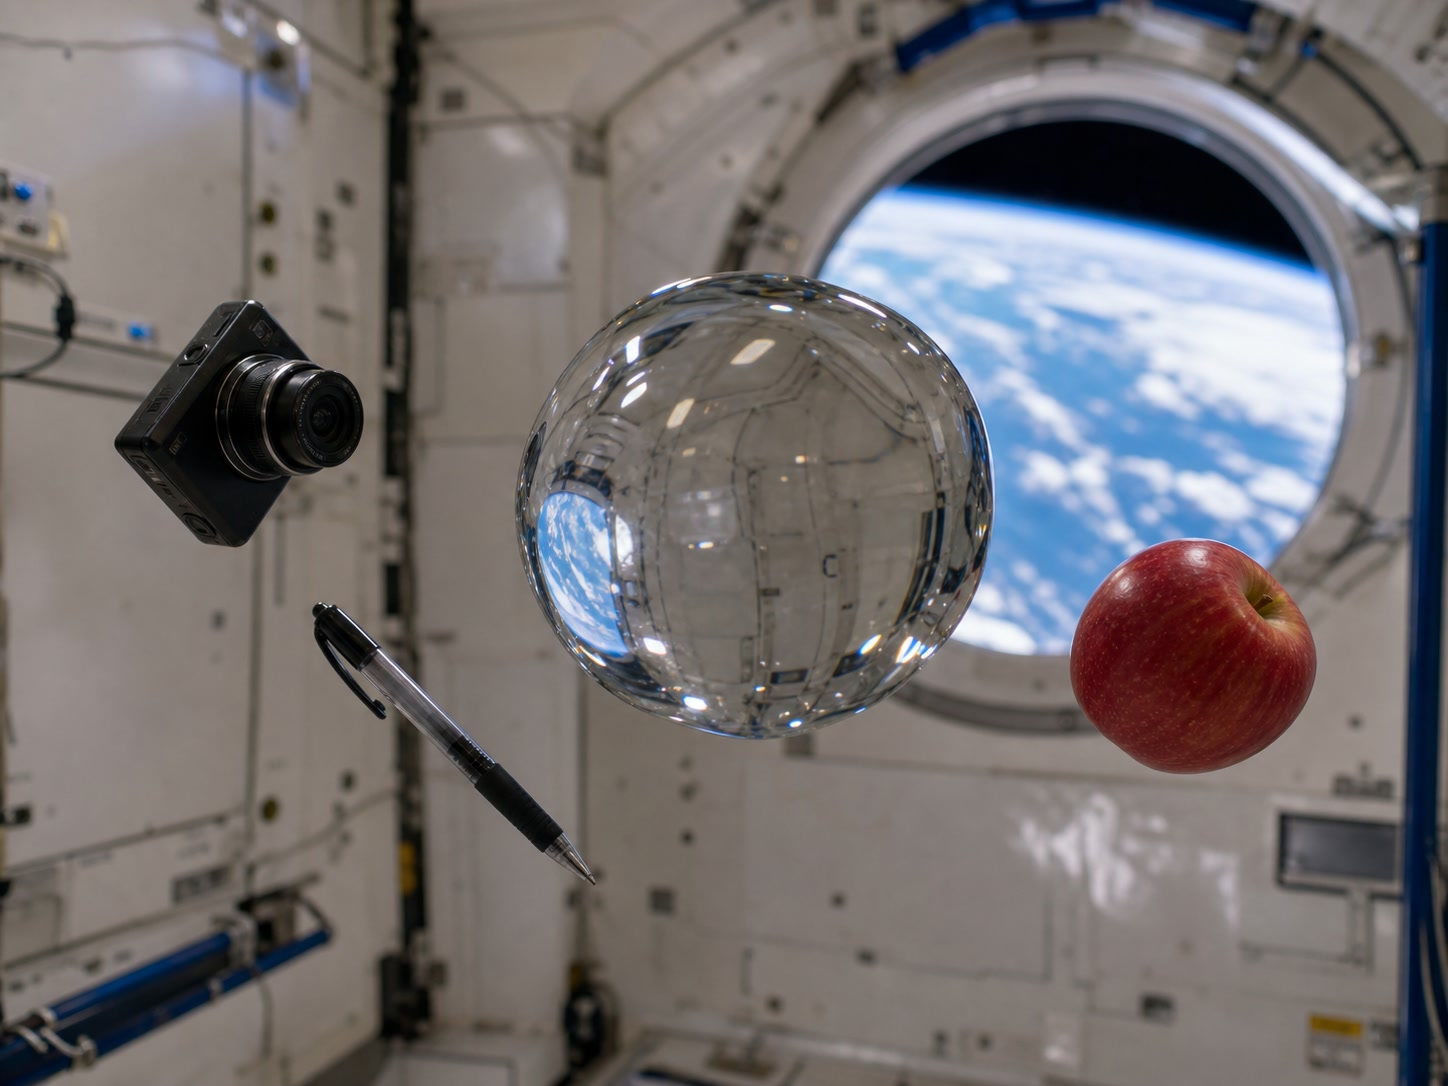
\includegraphics[width=0.5\linewidth]{images/book1/ai/g9-gravitation-weightless.jpg}

{\small 自由落体，日常可见：空间站及其中的一切一同绕地球下落，因此没有任何东西压向任何东西——相机、钢笔、苹果和水都飘浮起来。}
\end{omfigure}

\section{练习}

\begin{exercise}[$\star$]\label{exo:g9:gravitation:1}
写出\omterm{def:g9:gravitation:gravitation}{万有引力}定律——公式、\omterm{def:g6:measurement-in-science:measuring}{单位}，
并用文字叙述两个要点（\omterm{def:g3:measuring-mass:mass}{质量}与距离）。
\end{exercise}

\begin{exercise}[$\star$]\label{exo:g9:gravitation:2}
地球以 \qty{1}{N} 的力拉着苹果。苹果以多大的力
拉动地球？为什么两者中只有一个
会明显加速？
\end{exercise}

\begin{exercise}[$\star$]\label{exo:g9:gravitation:3}
两颗卫星分别绕地心运行，距地心分别为 $d$ 和 $2d$。
比较两者所受的\omterm{def:g9:gravitation:gravitation}{万有引力}
（\omterm{def:g3:measuring-mass:mass}{质量}相等）。那么在 $10 d$ 处呢？
\end{exercise}

\begin{exercise}[$\star$]\label{exo:g9:gravitation:4}
计算两位\omterm{def:g3:measuring-mass:mass}{质量}均为 \qty{80}{kg} 的舞伴之间的引力，
两人相距 \qty{0.5}{m}，并比较“浪漫”与
引力，谈谈你的看法。
\end{exercise}

\begin{exercise}[$\star$]\label{exo:g9:gravitation:5}
在山岳大炮的故事中，哪两个速率恰好
相等，才使炮弹绕行？用三个词说明什么是\omterm{def:g6:sun-earth-moon:axisorbit}{轨道}？
\end{exercise}

\begin{exercise}[$\star$]\label{exo:g9:gravitation:6}
“宇航员\omterm{def:g1:floating-and-sinking:words}{漂浮}，是因为那里没有\omterm{def:g4:weight-and-mass:weight}{重力}。”
请用炮弹的例子驳斥这一说法：空间站与
宇航员各自正在做什么？
\end{exercise}

\begin{exercise}[$\star$]\label{exo:g9:gravitation:7}
为什么\omterm{def:g9:gravitation:gravitation}{万有引力}——自然界中最弱的力——仍然
支配着宇宙？请依据本章给出两条理由。
\end{exercise}

\begin{exercise}[$\star$]\label{exo:g9:gravitation:8}
潮汐从何而来，大多数日子为何每天两次？
最大的潮汐何时出现？
\end{exercise}

\begin{exercise}[$\star\star$]\label{exo:g9:gravitation:9}
\omterm{def:g2:moon-in-the-sky:moon}{月球}（\omterm{def:g3:measuring-mass:mass}{质量} \qty{7.3e22}{kg}）绕地球运行，\omterm{def:g6:sun-earth-moon:axisorbit}{轨道}距离为 \qty{3.8e8}{m}，
地球\omterm{def:g3:measuring-mass:mass}{质量}为 \qty{5.97e24}{kg}。计算两者之间的引力，
全程使用科学计数法，并体会答案中
10 的幂次竟携带了多少位数字。
\end{exercise}

\begin{exercise}[$\star\star$]\label{exo:g9:gravitation:10}
在\omterm{def:g2:moon-in-the-sky:moon}{月球}表面，你的\omterm{def:g4:weight-and-mass:weight}{重力}缩减为地球上的
六分之一（回想那些蹦跳的宇航员）。运用定律的
两个“旋钮”——\omterm{def:g2:moon-in-the-sky:moon}{月球}较小的\omterm{def:g3:measuring-mass:mass}{质量}与较小的半径——
说明六分之一如何产生于一个比地球
轻八十倍的天体。
\end{exercise}

\begin{exercise}[$\star\star$]\label{exo:g9:gravitation:11}
水星绕太阳一周需 $88$ 天，海王星需 $165$ 年。
由平方反比律读出这一规律：引力随距离减弱，
对太阳的束缚有何影响，进而
对外\omterm{def:g4:solar-system:planet}{行星}家族的运行节奏有何影响？
\end{exercise}

\begin{exercise}[$\star\star\star$]\label{exo:g9:gravitation:12}
一颗地球静止卫星看似静止地悬于
赤道上某一点的上空——碟形天线始终不动。
请将这一现象与
\cref{prop:g9:gravitation:runs}：它的\omterm{def:g6:sun-earth-moon:axisorbit}{轨道}
周期应为多少、绕行方向如何，以及为何
这里所谓“悬停”，实为“与
自转的地球完全同步地下落”？
\end{exercise}

\section{问题：炮弹的遗产}

\begin{problem}[{周末问题——从果园到
轨道；苹果、火炮与月球，同用一条定律核算；
卫星发射看板}]\label{pb:g9:gravitation:1}
某个傍晚，在航天机构的科普咨询台前：一条定律，
$G = \qty{6.67e-11}{N.m^2/kg^2}$，地球\omterm{def:g3:measuring-mass:mass}{质量}
\qty{5.97e24}{kg}，地球半径 \qty{6.4e6}{m}。

\medskip\noindent\textbf{第一部分——苹果的核算。}
\begin{enumerate}
  \item 计算地球对一个 \qty{0.1}{kg} 的苹果在
        地表处的引力（两球心相距一个地球半径）。
  \item 苹果对地球的反作用力有多大？
        请说出定律对这种相互作用关系的称呼。
  \item 将苹果置于离地心为地球半径两倍的位置，
        引力会如何变化？
  \item 一位参观者问，公式为何使用的是
        到地球\emph{球心}的距离，而不是到
        地面的距离？请给出诚实的简短回答（整个
        \omterm{def:g4:solar-system:planet}{行星}都在拉动，其分散的引力合并起来
        效果等同于集中于球心——这是这位伟大作者
        本人历经数年才证明的定理）。
\end{enumerate}

\medskip\noindent\textbf{第二部分——发射看板。}
\begin{enumerate}[resume]
  \item 今日卫星\omterm{def:g3:measuring-mass:mass}{质量}为 \qty{2000}{kg}，其
        地表\omterm{def:g4:weight-and-mass:weight}{重力}由定律算得是多少？（或用下一章
        所说的捷径：约为每\omterm{def:g3:measuring-mass:units}{千克}
        \qty{9.8}{N}。）
  \item 在其工作\omterm{def:g6:sun-earth-moon:axisorbit}{轨道}上，距地心 \qty{1.28e7}{m}，
        即两倍地球半径处，引力仍对它施加的是地表\omterm{def:g4:weight-and-mass:weight}{重力}的
        几分之几？
  \item “那么高空仍有真实的引力吗？”
        请用数值加以确认，并说明卫星
        对这一引力做了什么，才没有
        坠毁。
  \item 发射解说词称“\omterm{def:g6:sun-earth-moon:axisorbit}{轨道}\omterm{def:g7:motion-average-speed:formula}{速度}须与
        下落相匹配”。请重述“山顶大炮”的故事，
        用两句话写入参观者宣传册。
\end{enumerate}

\medskip\noindent\textbf{第三部分——\omterm{def:g2:moon-in-the-sky:moon}{月球}的账目。}
\begin{enumerate}[resume]
  \item 若\omterm{def:g2:moon-in-the-sky:moon}{月球}距地心 \qty{3.8e8}{m}，
        则它运行于几个地球半径之外？（保留一位小数。）
  \item 由平方反比律可知，该处引力已减弱为
        地表引力的大约几分之几？
        （将上一问的结果平方。）
  \item 重述这一伟大洞见：果园中的苹果
        在第一秒内下落约 5 米；\omterm{def:g2:moon-in-the-sky:moon}{月球}
        每一秒都在向地球“下落”，仅约
        一毫米，却始终不会落到地面。请把两个事实
        联系起来，结合你的第 9、10 问的答案，说明为何
        \omterm{def:g2:moon-in-the-sky:moon}{月球}的下落要慢上数千倍，并说明它为何
        永无止境？
  \item 结束这场科普晚会：一条定律，三位
        主角——苹果、卫星与\omterm{def:g2:moon-in-the-sky:moon}{月球}。请写出
        看板上将三者统一起来的结语。
\end{enumerate}
\end{problem}
